\chapter{Stereoisomerie}

\begin{figure}[h!]
	\centering
	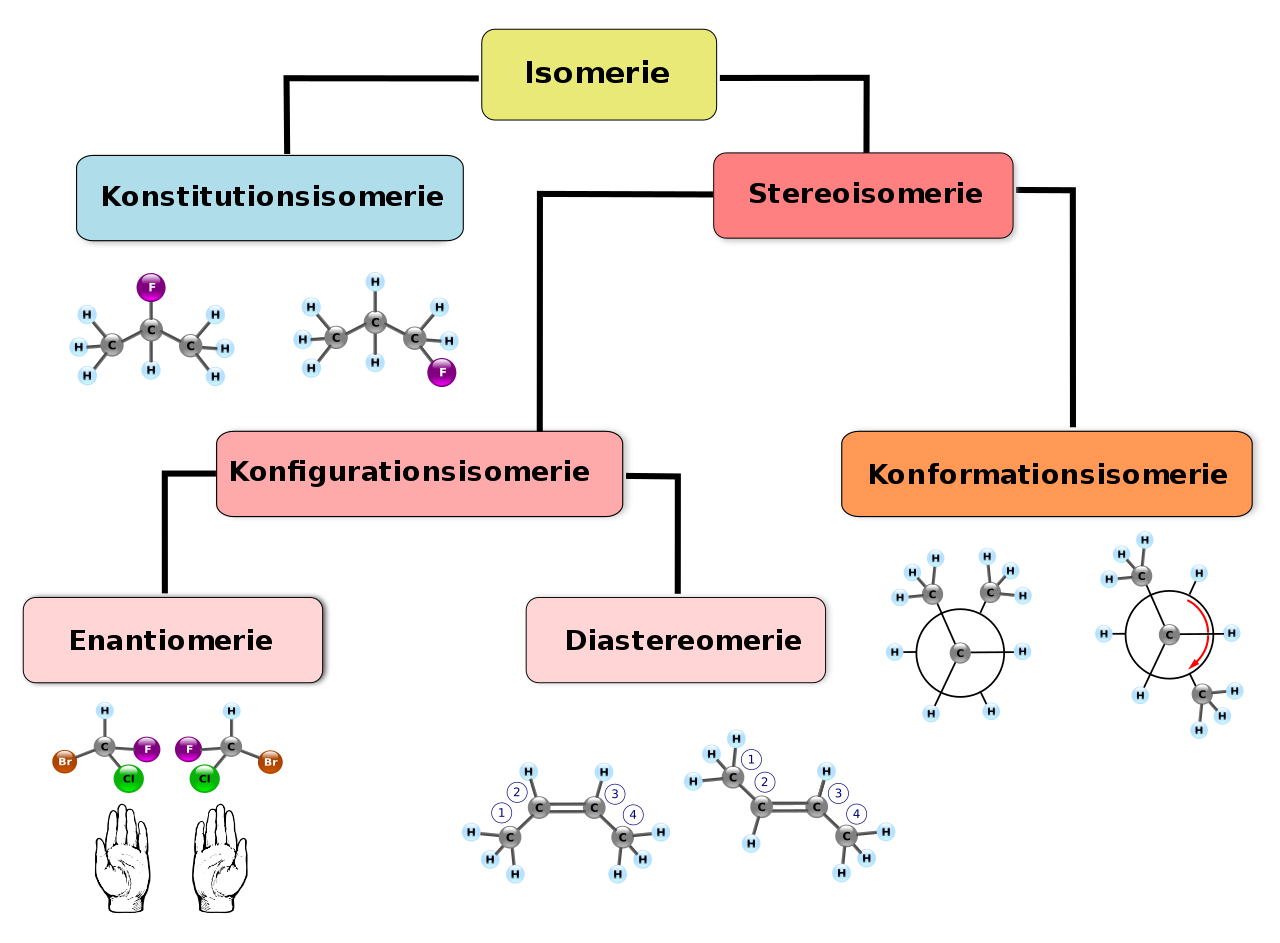
\includegraphics[width=0.75\linewidth]{img/isomerie}
	\caption{Übersicht der Isomerien}
	\label{fig:isomerie}
\end{figure}
\FloatBarrier

\begin{figure}[h!]
	\centering
	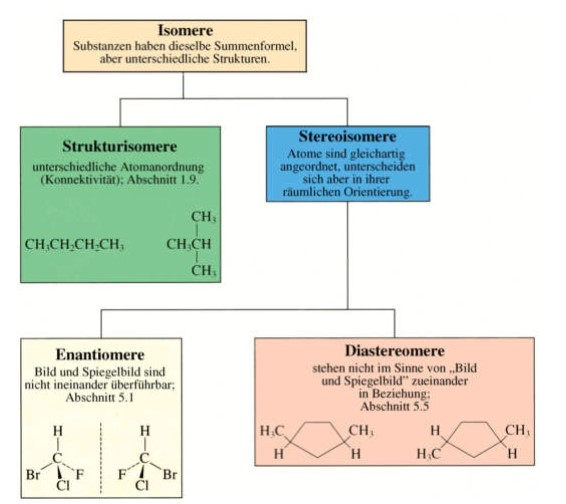
\includegraphics[width=0.75\linewidth]{img/isomerie2}
	\caption{Übersicht der Isomerien}
	\label{fig:isomerie2}
\end{figure}
\FloatBarrier

\section{Enantiomere}

\subsection{Begriffe der Enantiomere}

\textbf{{\large Chiralität:}} (griech. Händigkeit)\\
= jedes Objekt, das mit seinem Spiegelbild \textbf{nicht} zur Deckung gebracht werden kann ist chiral (nur das Molekül !)\\
$\rightarrow$ chirale Moleküle besitzen asymetrisch substituierte C-Atome als Stereozentrum
\begin{figure}[h!]
	\centering
	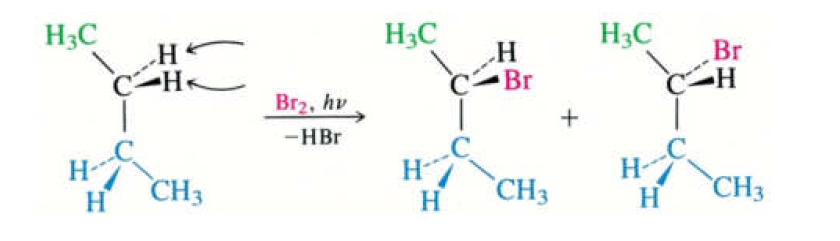
\includegraphics[width=0.75\linewidth]{img/chiral1}
	\caption{Beispielreaktion für Stereoisomere}
	\label{fig:ciral1}
\end{figure}
\FloatBarrier

\textbf{{\large Enantiomere:}} \\
= Moleküle verhalten sich wie Bild und Spiegelbild \linebreak 
 (aber nicht im Molekül selbst $\rightarrow$ sind chiral und besitzen keine molekulare Spiegelebene) \\
 $\rightarrow$ achirale Moleküle können keine Enantiomere sei, das sich Bild und Spiegelbild decken\\
 
\textbf{{\large Racemat:}} \\
= 50:50 Gemisch von Enantiomeren (L-/D-Moleküle, +/-)\\
$\rightarrow$ sind optisch inaktiv

\subsection{Unterscheidung der Enantiomere}
1. Röntgengrafische Kristallstrukturanalyse ("`Foto"')\\ 
\textbf{2. Polarimeter:} optische Rotation der Ebene des linear polarisierten Lichts


\begin{figure}[h!]
	\centering
	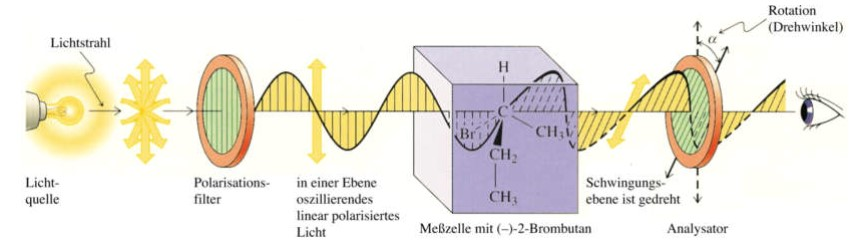
\includegraphics[width=0.75\linewidth]{img/polarimeter}
	\caption{optische Aktivität von chiralen Molekülen}
	\label{fig:polarimeter}
\end{figure}
\FloatBarrier
\begin{itemize}
	\item (+)- Enantiomer dreht sich im Uhrzeigersinn (dextrorotatorisch)
	\item (-)- Enantiomer dreht sich gegen Uhrzeigersinn (levorotatorisch)
\end{itemize}

Die Schwingungsebene des linear polarisierten Lichtes wird durch die optisch aktive Substanz am asymmetrisch substituierten C-Atom gedreht. \\
Je nachdem ob der Analysator mit oder gegen den Uhrzeigersinn dreht um das polarisierte Licht wahrzunehmen, erhält der Stoff die Bezeichnung (+/d) oder (-/l) \\

\textbf{Wichtig:} (+/d) $\neq$ D und (-/l) $\neq$ L\\

\textbf{{\large Spezifische Drehung:}}
\begin{flalign}
	\left[\alpha\right]^{\delta}_\lambda &= \frac{\alpha}{l*c}
\end{flalign}
\begin{itemize}
	\item $\left[\alpha\right]$... spezifische Drehung
	\item $\delta$... Temperatur in \si{\celsius}
	\item $\lambda$... Wellenlänge des einfallenden Lichtes
	\item $l$... Länge (in dm) der Messzelle (Küvette) 
	\item $c$... Konzentration in \si{\gram \per \milli \liter}
	\item $\alpha$... gemessene Rotation
\end{itemize}

\subsection{CIP- Sequenzregel}

\vspace*{3cm}
\textbf{{\large Fischerprojektion:}} \\
